% file: 3-9-connectivity/menger-theorem-case-I.tex
% Based on the proof of the book ``A First Course in Graph Theory'' by Gary Chartrand and Ping Zhang

\documentclass[tikz]{standalone}
\usetikzlibrary{positioning, decorations.pathmorphing}

\begin{document}
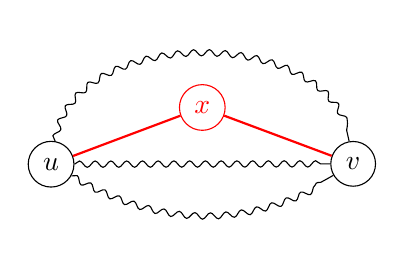
\begin{tikzpicture}[v/.style = {draw, circle, minimum size = 12pt},
    path/.style = {-, decorate, decoration = {snake, amplitude = .4mm, segment length = 2mm, post length = 1mm}}]
  \node (u) [v] {$u$};
  \node (x) [v, red, above right = 0.30cm and 1.50cm of u] {$x$};
  \node (v) [v, below right = 0.30cm and 1.50cm of x] {$v$};

  \path (u) edge[thick, red] (x)
	    edge[path] (v)
	    edge[path, bend left = 80] (v)
	    edge[path, bend right] (v)
	(x) edge[thick, red] (v);
\end{tikzpicture}
\end{document}